\section{Auswertung}
\label{sec:Auswertung}
In Tabelle \ref{tab:lit} sind die Literaturwerte der verwendeten Absorber eingetragen.
Die Literaturwerte für die Energien $E_\mathrm{K,Lit}$ wurden hierbei \cite{lit} entnommen.
Aus der Bragg-Bedingung ergibt sich durch Umformen und Ausnutzung des Zusammenhangs $\lambda=\frac{c}{\nu}=\frac{c\cdot h}{E}$ für den Glanzwinkel
\begin{equation}
	\theta=\arcsin{\frac{n\cdot \frac{c\cdot h}{E}}{2d}} \text{.}
\end{equation}
Die Abschirmkonstante wurde jeweils nach Formel \eqref{eqn:schirm} bestimmt.
\begin{table}
	\title{Literaturwerte zu den verwendeten Absorbern.}
	\label{tab:lit}
	\centering
\begin{tabular}{ccccc}
\toprule
Absorber & $Z$ & $E_\mathrm{K,Lit}$/$\si{\kilo\electronvolt}$ & $\theta_\mathrm{K,Lit}$ in Grad&$\sigma_\mathrm{K,Lit}$ \\
\midrule
Zn&30 & 9.65 & 18.6 & 3.57 \\
Ge&32 & 11.10 & 16.09 & 3.68 \\
Br&35 & 13.47& 13.21 & 3.85 \\
Zr&40 & 18.00 & 9.85 & 4.1 \\
Au; L-II-Kante&79 & 13.73 & 12.95 & 56.85 \\
Au; L-III-Kante&79 & 11.92 & 14.97 & 60.1 \\
\bottomrule
\end{tabular}
\end{table}

Zudem wurden nach \cite{UniG} die Literaturwerte für die Lage der Kennlinien bei einer Röntgenröhre mit Kupferanode verwendet, und erneut Glanzwinkel sowie Abschirmkonstante bestimmt. Die berechneten Theoriewerte finden sich in Tabelle \ref{tab2}.
\begin{table}
	\title{Literaturwerte zur Lage der Kennlinien des charakteristischen Spektrums der Rötgenröhre bei Verwendung einer Kupferanode ($Z=29$).}
	\centering
\begin{tabular}{cccc}
\toprule
 Kennlinie& $E_\mathrm{K,Lit}$/$\si{\electronvolt}$ & $\theta_\mathrm{K,Lit}$ in Grad&$\sigma_\mathrm{K,Lit}$ \\
\midrule
$K_\mathrm{\alpha,1}$& 8048.0 & 22.49 & 4.87 \\
$K_\mathrm{\alpha,2}$& 8028.0 & 22.55 & 4.9 \\
$K_\mathrm{\beta}$& 8905.0 & 20.22 & 3.6 \\
\bottomrule
\end{tabular}
\end{table}


\subsection{Überprüfung der Bragg-Bedingung}
\begin{figure}
	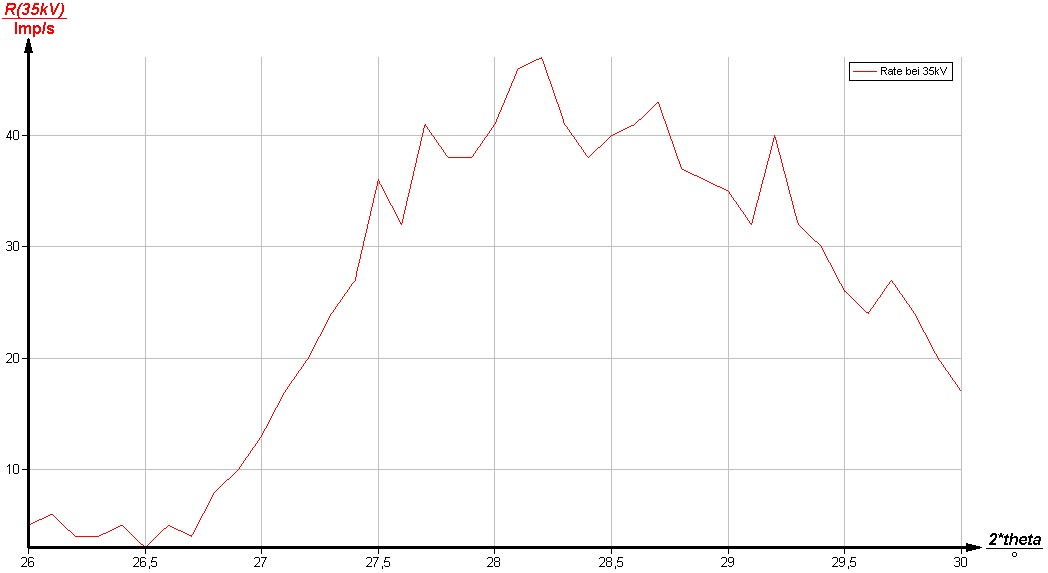
\includegraphics[width=1.0\textwidth]{nIKO_und_jULIAN_ÜLADS/breck.jpg}
	\caption{Gemessene Impulse in Abhängigkeit des abgelaufenen Winkels zur Überprüfung der Bragg-Bedingung.}
	\label{fig:braeck}
\end{figure}
Zur Überprüfung der Bragg-Bedindung wird das Maximum der Messkurve in Plot \ref{fig:braeck} bestimmt.
Um das Maximum möglichst genau bestimmen zu können sind die von der Messapparatur aufgenommenen Messdaten um das Maximum herum in Tabelle \ref{tab:bregg} aufgetragen.
Das Maximum wird aus der Tabelle entnommen zu $\alpha_\mathrm{max}=2\cdot \theta=28.2\textdegree$.
Da ein fester Kristallwinkel von $\theta=14\textdegree$ für die Messung eingestellt wurde, entspricht das gefundene Maximum fast genau dem Sollwinkel von $\alpha_\mathrm{Soll}=28\textdegree$ und die Bragg-Bedingung kann bestätigt werden.
\begin{table}
	\centering
	\caption{Aufgenommene Messdaten um das Maximum zur Bestätigung der Bragg-Bedingung.}
	\label{tab:bregg}
	\begin{tabular} {cc}
		\toprule
		$2 \cdot \theta$ /$\textdegree$ &Impulse/$\si{\second}$ \\%blaa angaben in grad?
\midrule
		27,7	&41,0\\
		27,8	&38,0\\
		27,9	&38,0\\
		28,0	&41,0\\
		28,1	&46,0\\
		28,2	&47,0\\
		28,3	&41,0\\
		28,4	&38,0\\
		28,5	&40,0\\
		28,6	&41,0\\
		28,7	&43,0\\
\bottomrule
	\end{tabular}
\end{table}

\FloatBarrier
\subsection{Das Emissionsspektrum der Kupfer-Röntgenröhre}
\begin{figure}
	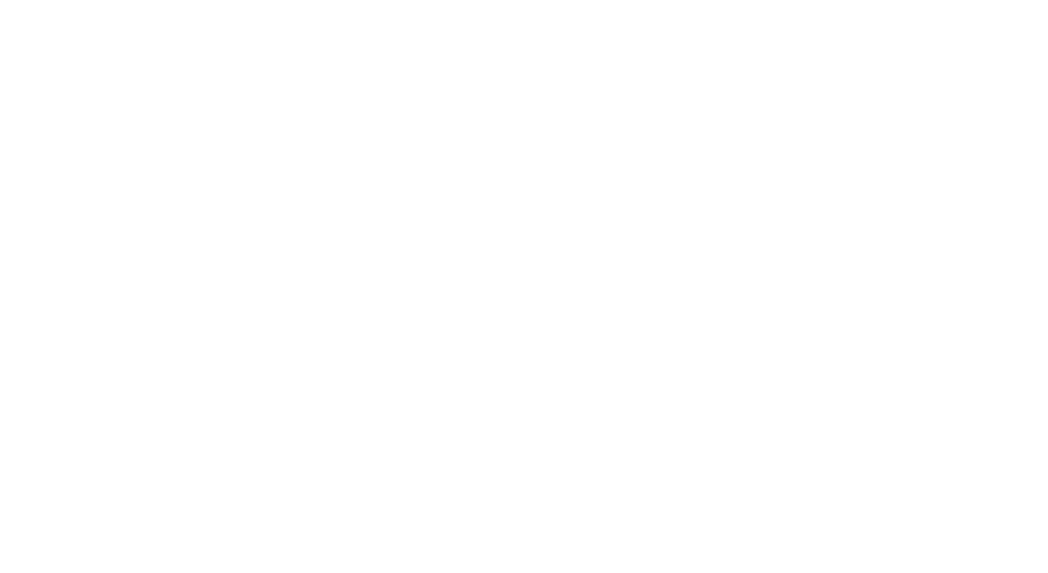
\includegraphics[width=0.95\textwidth]{nIKO_und_jULIAN_ÜLADS/Kupferemission.png}
	\caption{Aufgenommenes Emissionssspektrum der Cu-Röntgenröhre.}
	\label{fig:kupfer}
\end{figure}
\begin{figure}
	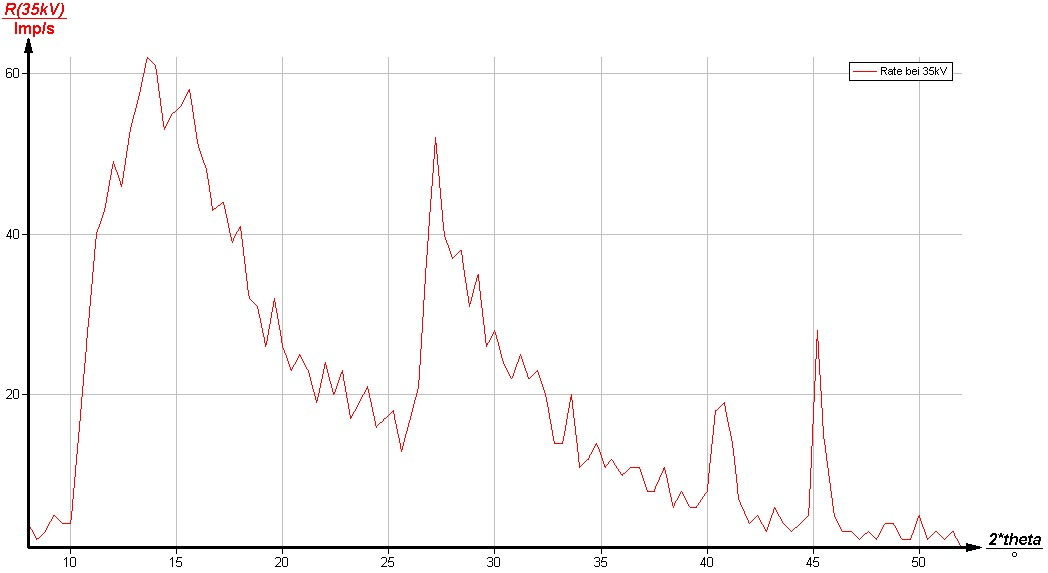
\includegraphics[width=1.0\textwidth]{nIKO_und_jULIAN_ÜLADS/Kupfaemmision.jpg}
	\caption{Aufgenommenes Emissionssspektrum der Kupfer-Röntgenröhre.}
	\label{fig:emissionlol}
\end{figure}




%%%%%%%%%%%%%%%%%%%%%%%%%%%%%%%%%%%%%%%%%%%%%%%%%%%%%%%%%%%%%%%%%%%%%%%%%%%%%%%%%%%%%%%%%%
\FloatBarrier
\subsection{Das Absorptionsspektrum}

\subsubsection{Absorber Zink}
\begin{figure}
	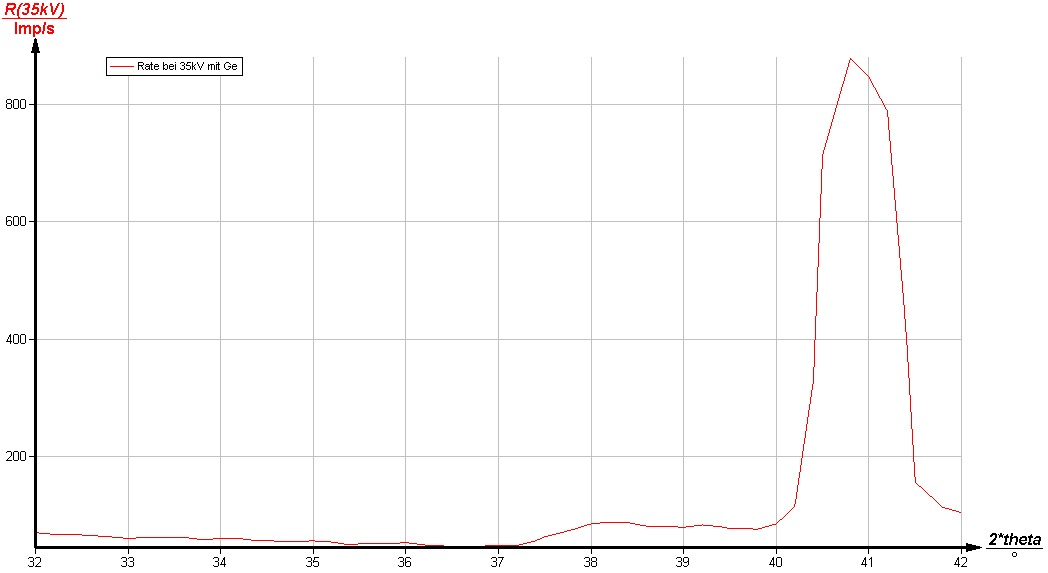
\includegraphics[width=1.0\textwidth]{nIKO_und_jULIAN_ÜLADS/zink.jpg}
	\caption{Aufgenommenes Absorptionsspektrum mit dem Absorber Zink.}
	\label{fig:zink_absorber}
\end{figure}
Das Absorptionsspektrum von Zink ist in Abbildung \ref{fig:zink_absorber} aufgetragen.
Es ergibt sich die K-Kante bei dem Winkel
\begin{equation*}
	\theta_{\mathrm{Zi,K}} = \SI{20,20}{\degree}
\end{equation*}
als Mittelwert von $\SI{20,0}{\degree}$ und $\SI{20,4}{\degree}$. 
Mit Formel \eqref{eqn:braggii} und dem Zusammenhang $E = \frac{\symup{hc}}{\lambda}$,
wobei $\symup{h}$
das Planck'sche Wirkungsquantum und $\symup{c}$ die Lichtgeschwindigkeit im Vakuum ist, lässt
sich die Absorptionsenergie durch
\begin{equation}
	\label{eqn:Absorptionsenergie}
	E = \frac{\symup{hc}}{2d\sin\theta}
\end{equation}
ermitteln.
Damit ergibt sich die Absorptionsenergie von Zink zu
\begin{equation*}
	E_{\mathrm{Zi,K}} = \SI{3,15432856(4)}{\kilo\electronvolt} \mathrm{.}
\end{equation*}

%%%%%%%%%%%%%%%%%%%%%%%%%%%%%%%%%%%%%%%%%%%%%%%%%%%%%
\FloatBarrier
\subsubsection{Absorber Germanium}
\begin{figure}
	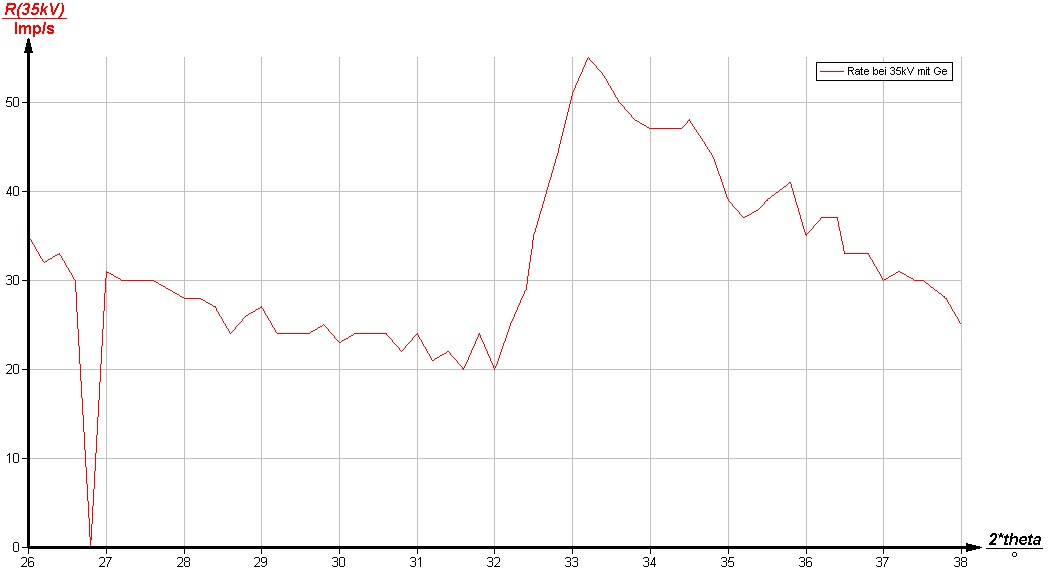
\includegraphics[width=1.0\textwidth]{nIKO_und_jULIAN_ÜLADS/germanium.jpg}
	\caption{Aufgenommenes Absorptionsspektrum mit dem Absorber Germanium.}
	\label{fig:germanium_absorber}
\end{figure}
Das Absorptionsspektrum von Germanium ist in Abbildung \ref{fig:germanium_absorber}
dargestellt. Es wird die K-Kante als Mittelwert von $\theta_1 = \SI{16,0}{\degree}$ und
$\theta_2 = \SI{16,6}{\degree}$ zu
\begin{equation*}
	\theta_{\mathrm{Ge,K}} = \SI{16,30}{\degree}
\end{equation*}
bestimmt. Damit ergibt sich nach Formel \eqref{eqn:Absorptionsenergie} die Absorptionsenergie
von Germanium zu
\begin{equation*}
	E_{\mathrm{Ge,K}} = \SI{5.51571723(7)}{\kilo\electronvolt} \mathrm{.}
\end{equation*}
Weiterhin lässt sich mit Formel \eqref{eqn:} die Abschirmzahl von Germanium zu
\begin{equation*}
	\sigma_{\mathrm{Ge,K}} = 2
\end{equation*}
berechnen.

%%%%%%%%%%%%%%%%%%%%%%%%%%%%%%%%%%%%%%%%%%%%%%%%%%%%%%%%%
\FloatBarrier
\subsubsection{Absorber Brom}
\begin{figure}
	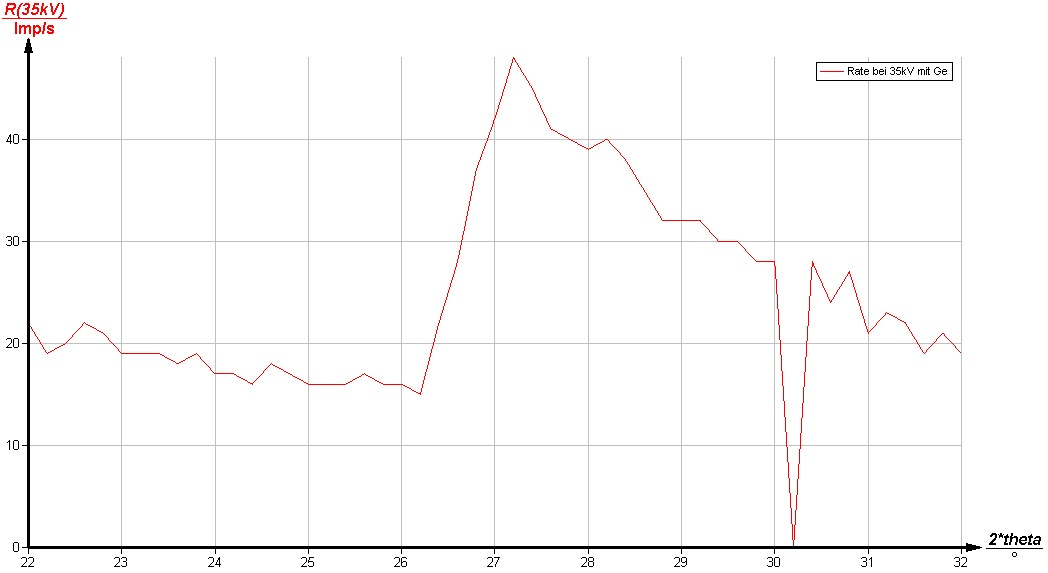
\includegraphics[width=1.0\textwidth]{nIKO_und_jULIAN_ÜLADS/brom.jpg}
	\caption{Aufgenommenes Absorptionsspektrum mit dem Absorber Brom.}
	\label{fig:brom_absorber}
\end{figure}
Das Absorptionsspektrum von Brom ist in Abbildung \ref{fig:brom_absorber} dargestellt.
Es ergibt sich wieder analog wie bei Zink und Germanium die K-Kante als Mittelwert von 
$\SI{13,1}{\degree}$ und $\SI{13,6}{\degree}$ zu
\begin{equation*}
	\theta_{\mathrm{Br,K}} = \SI{13,35}{\degree} \mathrm{.}
\end{equation*}
Damit ergbt sich die Absorptionsenergie mit Formel \eqref{eqn:Absorptionsenergie} zu
\begin{equation*}
	E_{\mathrm{Br,K}} = \SI{4,36075213(5)}{\kilo\electronvolt} \mathrm{.}
\end{equation*}

\FloatBarrier
\subsubsection{Absorber Zirkonium}
\begin{figure}
	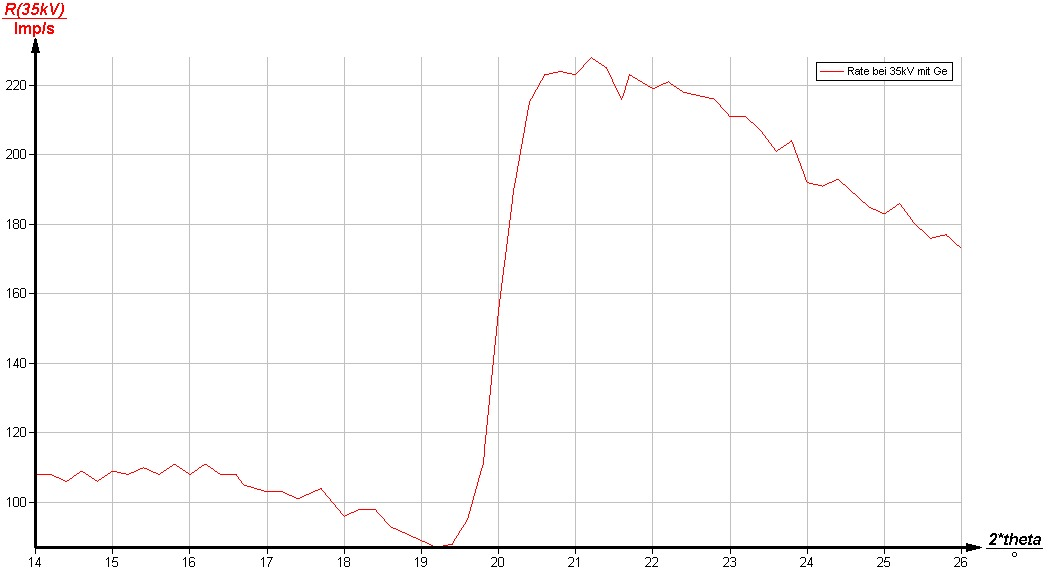
\includegraphics[width=1.0\textwidth]{nIKO_und_jULIAN_ÜLADS/zirkonium.jpg}
	\caption{Aufgenommenes Absorptionsspektrum mit dem Absorber Zirkonium.}
	\label{fig:zirkonium_absorber}
\end{figure}
In Abbildung \ref{fig:zirkonium_absorber} ist das Absorptionsspektrum von Zirkonium 
dargestellt.
Es ergibt sich die K-Kante bei
\begin{equation*}
	\theta_{\mathrm{Zr,K}} = \SI{10,00}{\degree} \mathrm{,}
\end{equation*}
als Mittelwert von $\SI{9,7}{\degree}$ und $\SI{10,3}{\degree}$.
Es ergibt sich die Absorptionsenergie von Zirkonium zu
\begin{equation*}
	E_{\mathrm{Zr,K}} = \SI{5.65797625(7)}{\kilo\electronvolt} \mathrm{.}
\end{equation*}
Gold 7325.79726+/-0.00009 zweite: 6328.26238+/-0.00008

\FloatBarrier
\subsubsection{Absorber Gold}
\begin{figure}
	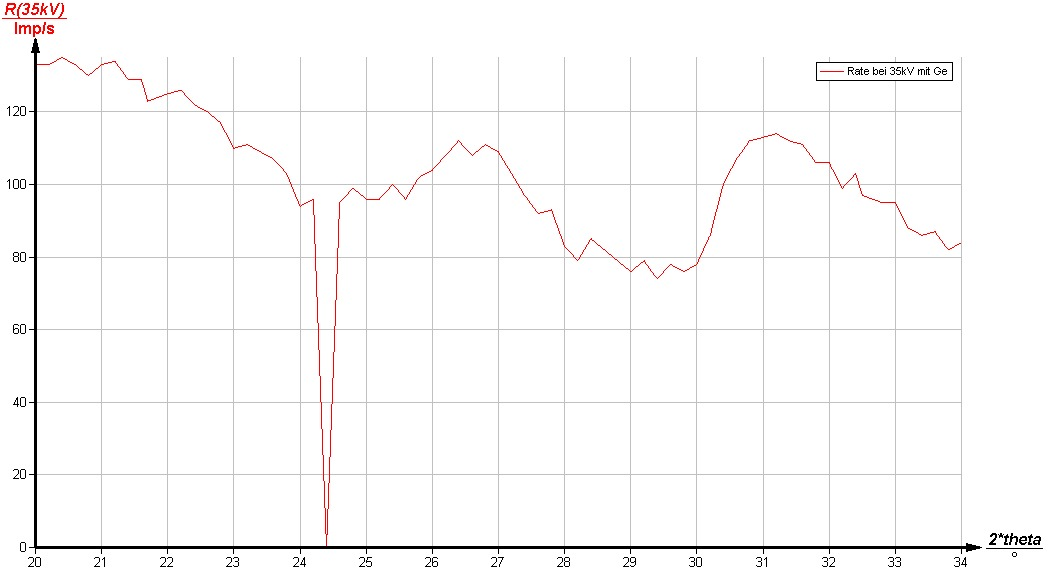
\includegraphics[width=1.0\textwidth]{nIKO_und_jULIAN_ÜLADS/gold.jpg}
	\caption{Aufgenommenes Absorptionsspektrum mit dem Absorber Gold.}
	\label{fig:gold_absorber}
\end{figure}
Das Absorptionsspektrum von Gold ist in Abbildung \ref{fig:gold_absorber} dargestellt.
Es werden die L-Kanten bei
\begin{gather*}
	\theta_{\mathrm{Au,L}_{\mathrm{II}}} = \SI{13,00}{\degree} \mathrm{,} \\
	\theta_{\mathrm{Au,L}_{\mathrm{III}}} = \SI{15,20}{\degree} \mathrm{,} \\
\end{gather*}
als Mittelwert von $\SI{12,8}{\degree}$ und $\SI{13,2}{\degree}$ bzw. $\SI{14,9}{\degree}$
und $\SI{15,5}{\degree}$ abgelesen.
Es ergeben sich mit Formel \eqref{eqn:Absorptionsenergie} wieder die Absorptionsenergien von
Gold zu
\begin{gather*}
	E_{\mathrm{Au,L}_{\mathrm{II}}} = \SI{7,32579726(9)}{\kilo\electronvolt} \mathrm{,} \\
	E_{\mathrm{Au,L}_{\mathrm{III}}} = \SI{6,32826238(8)}{\kilo\electronvolt} \mathrm{.} \\
\end{gather*}
